% ============================================================
%  hw2_sol.tex   --  MATH 6660, Homework 2.
%
%  RULE: nothing in this document goes beyond the class lectures.
%  Every step is tagged with the lecture it comes from.  Anything that
%  would go outside them is wrapped in \outside{}{} and prints as a red
%  labelled box, so it is visible in the PDF.
%
%  Build: pdflatex hw2_sol.tex   (twice, for cross-references)
% ============================================================
\documentclass[11pt]{article}
\usepackage[letterpaper,margin=1in]{geometry}
\usepackage[T1]{fontenc}
\usepackage{amsmath,amssymb,amsthm}
\usepackage{booktabs}
\usepackage{graphicx}
\usepackage{caption}
\usepackage{enumitem}
\usepackage{bm}
\usepackage{tikz}
\usetikzlibrary{arrows.meta}
\usepackage{xcolor}
\usepackage[colorlinks=true,linkcolor={blue!45!black},pdfborder={0 0 0}]{hyperref}
\usepackage{pdfcomment}

\newcommand{\dx}{\,\mathrm{d}x}
\newcommand{\norm}[1]{\lVert #1\rVert}
\newcommand{\abs}[1]{\lvert #1\rvert}
\newcommand{\Kmat}{\bm{K}}
\newcommand{\Th}{\mathcal{T}_h}
\setlength{\parindent}{0pt}

% ---- provenance tag: which lecture a step comes from ------------------
\newcommand{\src}[1]{{\small\color{black!55}\textsf{[#1]}}}

% ---- anything outside the lectures is boxed and labelled -------------
\newcommand{\outside}[2]{%
  \par\smallskip\noindent
  \fcolorbox{red!65!black}{red!4}{%
    \parbox{0.955\linewidth}{\small
      \textbf{\color{red!65!black}NOT FROM LECTURE --- #1}\par\smallskip #2}}%
  \par\smallskip}

% ---- bullets ---------------------------------------------------------
\newlist{steps}{itemize}{1}
\setlist[steps]{label=\textbullet, leftmargin=1.25em, topsep=3pt,
                itemsep=4pt, parsep=0pt}

% ---- hover tooltips on cross-references ------------------------------
\makeatletter
\newcommand{\settip}[2]{\expandafter\gdef\csname femtip@#1\endcsname{#2}}
\newcommand{\gettip}[1]{%
  \ifcsname femtip@#1\endcsname\csname femtip@#1\endcsname\else equation \ref{#1}\fi}
\newcommand{\eqr}[1]{\pdftooltip{\eqref{#1}}{\gettip{#1}}}
\makeatother

\settip{eq:ode}{Periodic BVP: minus u double prime plus q u = f, u and u prime matching at the two ends, q positive}
\settip{eq:mult}{Multiply the ODE by v and integrate over the interval}
\settip{eq:parts}{One integration by parts: integral of u prime v prime plus q u v, minus the boundary bracket, equals integral of f v}
\settip{eq:bdry}{Boundary bracket collapses to u prime at pi times the jump of v across the two ends}
\settip{eq:space}{V is the set of v with v and v prime square integrable and v matching at the two ends}
\settip{eq:var}{Variational problem: find u in V with the bilinear expression equal to the integral of f v, for all v in V}
\settip{eq:fem}{FEM: find U in Vh satisfying the same identity for all v in Vh}
\settip{eq:go}{Galerkin orthogonality: the bilinear expression in e and v vanishes for all v in Vh}
\settip{eq:enorm}{Energy norm: square root of the integral of v prime squared plus q v squared}

\settip{eq:mesh}{Uniform mesh: h = 2 pi over (M+1), nodes x j = -pi + j h}
\settip{eq:Vh}{Vh is the set of v in V that are linear on each element: continuous piecewise linears}
\settip{eq:hat}{Interior hat function: rises from 0 to 1 on the element to the left of node j, falls back to 0 on the element to the right}
\settip{eq:hat0}{The hat at the glued node: its right half sits on the first element, its left half on the last}
\settip{eq:span}{Vh is the span of the M+1 hat functions, so its dimension is M+1}
\settip{eq:trial}{Trial function U is the sum of xi j times phi j, and xi j is the nodal value of U}
\settip{eq:sys}{Linear system K xi = b of size M+1, with K i j the pairing of two hat functions and b i the integral of f times phi i}

\settip{eq:cauchy}{Cauchy inequality: the absolute value of the integral of v prime w prime plus q v w is at most the product of the two energy norms}
\settip{eq:split}{Split the error: e = (u minus v) plus (v minus U), where the second piece lies in Vh}
\settip{eq:opt}{Optimality: the energy norm of u minus U is at most that of u minus v, for every v in Vh}
\settip{eq:interp}{Lecture 7 interpolation estimate: energy norm of u minus its interpolant is at most C times the norm of h u double prime}
\settip{eq:l2int}{L2 bound on the interpolation error: its L2 norm is at most h times the L2 norm of its derivative}
\settip{eq:apriori}{A priori estimate: energy norm of u minus U is at most C h times the L2 norm of u double prime}

\settip{eq:dual}{Dual problem: minus phi double prime plus q phi = e, with periodic conditions on phi and phi prime}
\settip{eq:esq}{The squared L2 norm of e written as an integral pairing e with phi}
\settip{eq:go2}{Galerkin orthogonality used with the slot filled by the interpolant of phi}
\settip{eq:phibd}{L2 norm of phi is at most the L2 norm of e divided by q min}
\settip{eq:stab}{Stability: L2 norm of phi double prime is at most C S times the L2 norm of e}
\settip{eq:l2err}{A priori L2 estimate: the L2 norm of u minus U is at most a constant times h squared times the L2 norm of u double prime}

\begin{document}

\begin{center}
  {\large\textbf{MATH 6660 --- Homework 2}}\\[0.2em]
  Hasan
\end{center}
\vspace{0.2em}

{\small\color{black!60}
Each step is tagged with the lecture it comes from. Anything outside the
lectures is boxed and labelled \textbf{NOT FROM LECTURE}.}

\vspace{0.8em}
% ==================================================================
\section*{Problem 1}

\textbf{Problem.} For
\begin{equation}\label{eq:ode}
  \textbf{ODE}:\ -u''+q(x)\,u=f(x),
  \qquad
  \textbf{BC1}:\ u(-\pi)=u(\pi),
  \qquad
  \textbf{BC2}:\ u'(-\pi)=u'(\pi),
\end{equation}
with $q>0$ on $[-\pi,\pi]$: derive a Galerkin orthogonality expression, and
deduce from it an appropriate energy norm.

% ------------------------------------------------------------------
\subsection*{Step 1 --- variational form \ \src{Lecture 1}}

\begin{steps}
\item Multiply \eqr{eq:ode} by a test function $v$ and integrate:
\begin{equation}\label{eq:mult}
  \int_{-\pi}^{\pi}\bigl(-u''+q\,u\bigr)v\dx=\int_{-\pi}^{\pi}f\,v\dx .
\end{equation}

\item Integrate the $u''$ term by parts once:
\begin{equation}\label{eq:parts}
  \int_{-\pi}^{\pi}\bigl(u'v'+q\,u\,v\bigr)\dx
  \;-\;\bigl[\,u'v\,\bigr]_{-\pi}^{\pi}
  \;=\;\int_{-\pi}^{\pi}f\,v\dx .
\end{equation}

\item Collapse the boundary bracket with \textbf{BC2}, $u'(-\pi)=u'(\pi)$:
\begin{equation}\label{eq:bdry}
  \bigl[\,u'v\,\bigr]_{-\pi}^{\pi}
   = u'(\pi)\,v(\pi)-u'(-\pi)\,v(-\pi)
   = u'(\pi)\bigl[\,v(\pi)-v(-\pi)\,\bigr].
\end{equation}

\item It vanishes exactly when $v$ is periodic. That requirement defines the
      space:
\begin{equation}\label{eq:space}
  V=\Bigl\{\,v:\ \int_{-\pi}^{\pi}\bigl(v^{2}+(v')^{2}\bigr)\dx<\infty,
    \ \ v(-\pi)=v(\pi)\,\Bigr\}.
\end{equation}

\item \textbf{Variational problem:} find $u\in V$ such that
\begin{equation}\label{eq:var}
  \int_{-\pi}^{\pi}\bigl(u'v'+q\,u\,v\bigr)\dx=\int_{-\pi}^{\pi}f\,v\dx
  \qquad\forall\,v\in V .
\end{equation}

\item \textbf{BC1} essential --- built into $V$ in \eqr{eq:space}.
      \textbf{BC2} natural --- not imposed on $V$; it is what collapsed
      \eqr{eq:bdry}.
      \src{Lecture 6, \textcircled{\scriptsize1}\,\textcircled{\scriptsize2}}

\item Trial space $=$ test space $=V$.
\end{steps}

% ------------------------------------------------------------------
\subsection*{Step 2 --- the finite element method \ \src{Lecture 6}}

\begin{steps}
\item Take any $V_h\subset V$. Find $U\in V_h$ such that
\begin{equation}\label{eq:fem}
  \int_{-\pi}^{\pi}\bigl(U'v'+q\,U\,v\bigr)\dx=\int_{-\pi}^{\pi}f\,v\dx
  \qquad\forall\,v\in V_h .
\end{equation}
\end{steps}

% ------------------------------------------------------------------
\subsection*{Step 3 --- Galerkin orthogonality \ \src{Lecture 6}}

\begin{steps}
\item $V_h\subset V$, so \eqr{eq:var} holds in particular for every $v\in V_h$.
\item Subtract \eqr{eq:fem} from it --- the right-hand sides cancel.
\item With $e:=u-U$:
\begin{equation}\label{eq:go}
  \boxed{\;\int_{-\pi}^{\pi}\bigl(e'v'+q\,e\,v\bigr)\dx=0
         \qquad\forall\,v\in V_h\;}
\end{equation}
\item The $v$ in \eqr{eq:go} is a \textbf{dummy slot}. The statement is that
      this integral vanishes whenever the slot holds a member of $V_h$ ---
      whatever we happen to call it. Later steps fill that slot with specific
      members.
\end{steps}

% ------------------------------------------------------------------
\subsection*{Step 4 --- energy norm, read off \eqr{eq:go} \ \src{Lecture 6}}

\begin{steps}
\item The integrand of \eqr{eq:go} pairs \emph{two} functions, $e$ and $v$:
\[
  e'v'+q\,e\,v .
\]

\item The energy norm is that same integrand with \textbf{both factors the same
      function}. Put $v$ in place of both:
\[
  \int_{-\pi}^{\pi}\bigl(v'v'+q\,v\,v\bigr)\dx
   =\int_{-\pi}^{\pi}\Bigl[\,(v')^{2}+q\,v^{2}\,\Bigr]\dx\;\ge\;0 .
\]
      \src{Lecture 6 does exactly this for $-(au')'=f$: Galerkin orthogonality
      there is $\int_0^1 a\,(u-U)'v'\dx=0$, and the energy norm is
      $\norm{v}_{E}^{2}=\int_0^1 a\,v'v'\dx$ --- the same integrand with both
      factors $v$}

\item Hence
\begin{equation}\label{eq:enorm}
  \boxed{\;\norm{v}_{E}
    :=\left(\int_{-\pi}^{\pi}\Bigl[\,(v')^{2}+q\,v^{2}\,\Bigr]\dx\right)^{1/2}\;}
\end{equation}

\item Why this is the \emph{appropriate} one: it was not chosen. It is the
      integrand of \eqr{eq:go} itself, which came out of the integration by
      parts in Step~1. Change the ODE and the integrand changes, so the norm
      changes with it.

\item It is a norm: both terms of the integrand are non-negative, so
      $\norm{v}_{E}=0$ forces $\int(v')^{2}\dx=0$ \emph{and}
      $\int q\,v^{2}\dx=0$; with $q>0$ this gives $v\equiv0$.
      \src{Lecture 3 runs the same argument with $a\ge a_{1}>0$}

\item Why the problem states $q>0$: with $q\equiv0$ this would be only a
      \emph{seminorm}. Periodic conditions leave constants in \eqr{eq:space},
      and a constant has $v'\equiv0$ but $v\not\equiv0$. The $q\,v^{2}$ term is
      what removes them.
\end{steps}

\clearpage
% ==================================================================
\section*{Problem 2}

\textbf{Problem.} Develop a CG(1) method for \eqr{eq:ode}, clearly stating the
appropriate spaces, trial, test, and basis functions.

{\small\color{black!60}
Everything below is the Lecture 3--4 construction applied to \eqr{eq:ode}. Two
things differ from the lecture, and both are forced by this problem rather than
imported from anywhere: the bilinear expression carries the extra $q\,uv$ term
(from Problem 1, Step 1), and the boundary conditions are periodic instead of
Dirichlet.}

% ------------------------------------------------------------------
\subsection*{Step 1 --- mesh
  \ \src{Lecture 3: defines a mesh $\Th$ on the interval with
         $h_j=x_j-x_{j-1}$, spacing allowed to vary}}

\begin{steps}
\item Take the uniform mesh of the hint:
\begin{equation}\label{eq:mesh}
  h=\frac{2\pi}{M+1},\qquad x_j=-\pi+j\,h,\quad j=0,1,\dots,M+1 .
\end{equation}
\item So $x_0=-\pi$ and $x_{M+1}=\pi$. Elements $I_j=[x_{j-1},x_j]$,
      $j=1,\dots,M+1$ --- that is $M+1$ elements.
\item \textbf{BC1 says $x_0$ and $x_{M+1}$ are the same point of the domain.}
      So there are $M+1$ \emph{distinct} nodes, not $M+2$.
\end{steps}

% ------------------------------------------------------------------
\subsection*{Step 2 --- the space $V_h$
  \ \src{Lecture 3: ``the simplest $V_h\subset V$ is the space of continuous
         piecewise linear polynomials on $\Th$'' --- this is CG(1)}}

\begin{steps}
\item Continuous piecewise linears on this mesh:
\begin{equation}\label{eq:Vh}
  V_h=\bigl\{\,v\in V:\ v|_{I_j}\ \text{is linear},\ j=1,\dots,M+1\,\bigr\}.
\end{equation}
\item $V_h\subset V$ by construction. That containment is what Step 3 of
      Problem 1 needed in order to subtract, so Galerkin orthogonality
      \eqr{eq:go} applies here unchanged.
\item $\dim V_h=M+1$: a continuous piecewise linear on $M+1$ elements carries
      $M+2$ nodal values, and BC1 identifies the two end values as one.
      \src{Lecture 4 gets $\dim V_h=M$ for Dirichlet: there the two end values
           are \emph{deleted}; here they are \emph{merged}}
\end{steps}

% ------------------------------------------------------------------
\subsection*{Step 3 --- basis functions
  \ \src{Lecture 3--4: the hat function $\varphi_j$ associated with node $x_j$,
         and $V_h=\operatorname{span}\{\varphi_1,\dots,\varphi_M\}$}}

\begin{steps}
\item Interior nodes $j=1,\dots,M$ --- the lecture's hat, with $h_j\equiv h$:
\begin{equation}\label{eq:hat}
  \varphi_j(x)=
  \begin{cases}
    \dfrac{x-x_{j-1}}{h}, & x_{j-1}\le x\le x_j,\\[2ex]
    \dfrac{x_{j+1}-x}{h}, & x_j\le x\le x_{j+1},\\[1.2ex]
    0, & \text{otherwise.}
  \end{cases}
\end{equation}

\item At the glued node, one hat whose two halves sit at the two ends of the
      interval:
\begin{equation}\label{eq:hat0}
  \varphi_0(x)=
  \begin{cases}
    \dfrac{x_1-x}{h}, & x_0\le x\le x_1,\\[2ex]
    \dfrac{x-x_M}{h}, & x_M\le x\le x_{M+1},\\[1.2ex]
    0, & \text{otherwise.}
  \end{cases}
\end{equation}

\item Check: $\varphi_0(x_0)=1$ and $\varphi_0(x_{M+1})=1$ --- the same value at
      the same point of the domain, so $\varphi_0$ is continuous there and
      $\varphi_0\in V_h$. Nodal property $\varphi_i(x_j)=\delta_{ij}$ holds for
      all $i,j=0,\dots,M$.

\item Hence the basis, one hat per distinct node:
\begin{equation}\label{eq:span}
  V_h=\operatorname{span}\{\varphi_0,\varphi_1,\dots,\varphi_M\},
  \qquad \dim V_h=M+1 .
\end{equation}
\end{steps}

\begin{center}
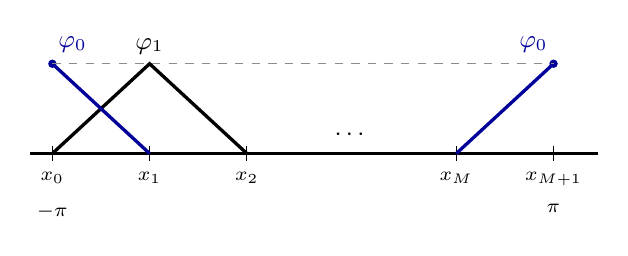
\begin{tikzpicture}[>=Latex,scale=0.95]
  \draw[thick] (-0.3,0) -- (7.3,0);
  \foreach \i/\lab in {0/{x_0},1.3/{x_1},2.6/{x_2},5.4/{x_M},6.7/{x_{M+1}}}{
     \draw (\i,-0.1) -- (\i,0.1);
     \node[below,font=\scriptsize] at (\i,-0.12) {$\lab$};}
  \node[font=\small] at (4.0,0.25) {$\cdots$};
  \node[below,font=\scriptsize] at (0,-0.55) {$-\pi$};
  \node[below,font=\scriptsize] at (6.7,-0.55) {$\pi$};
  % interior hat
  \draw[very thick] (0,0) -- (1.3,1.2) -- (2.6,0);
  \node[above,font=\small] at (1.3,1.2) {$\varphi_1$};
  % wrap hat
  \draw[very thick,blue!60!black] (0,1.2) -- (1.3,0);
  \draw[very thick,blue!60!black] (5.4,0) -- (6.7,1.2);
  \fill[blue!60!black] (0,1.2) circle (1.6pt);
  \fill[blue!60!black] (6.7,1.2) circle (1.6pt);
  \draw[dashed,black!45] (0,1.2) -- (6.7,1.2);
  \node[above right,font=\small,blue!60!black] at (-0.05,1.22) {$\varphi_0$};
  \node[above left,font=\small,blue!60!black]  at (6.75,1.22) {$\varphi_0$};
\end{tikzpicture}
\par\smallskip
{\small The two blue halves are \emph{one} basis function $\varphi_0$, carrying
the single unknown $\xi_0$: $x_0$ and $x_{M+1}$ are the same point of the
domain. $\varphi_1$ is an ordinary interior hat.}
\end{center}

% ------------------------------------------------------------------
\subsection*{Step 4 --- trial and test functions
  \ \src{Lecture 3: any $U\in V_h$ is uniquely $U=\sum_j\xi_j\varphi_j$;
         Lecture 4: take $v=\varphi_i$}}

\begin{steps}
\item \textbf{Trial:}
\begin{equation}\label{eq:trial}
  U(x)=\sum_{j=0}^{M}\xi_j\,\varphi_j(x),\qquad \xi_j=U(x_j).
\end{equation}
\item \textbf{Test:} $v=\varphi_i$, \ $i=0,1,\dots,M$.
\item Trial space $=$ test space $=V_h$ --- this is what makes it Galerkin.
\end{steps}

% ------------------------------------------------------------------
\subsection*{Step 5 --- the linear system
  \ \src{Lecture 4: substitute the expansion into the FEM statement, take
         $v=\varphi_i$, obtain $\Kmat\bm{\xi}=\bm{b}$ with
         $K_{ij}=\int a\,\varphi_i'\varphi_j'\dx$, $b_i=\int f\varphi_i\dx$}}

\begin{steps}
\item Put \eqr{eq:trial} into the FEM statement \eqr{eq:fem} and take
      $v=\varphi_i$:
\[
  \sum_{j=0}^{M}\xi_j
    \int_{-\pi}^{\pi}\bigl(\varphi_i'\varphi_j'+q\,\varphi_i\varphi_j\bigr)\dx
  =\int_{-\pi}^{\pi}f\,\varphi_i\dx ,
  \qquad i=0,1,\dots,M .
\]
\item That is an $(M+1)\times(M+1)$ system:
\begin{equation}\label{eq:sys}
  \boxed{\;\Kmat\bm{\xi}=\bm{b},\qquad
    K_{ij}=\int_{-\pi}^{\pi}\bigl(\varphi_i'\varphi_j'+q\,\varphi_i\varphi_j\bigr)\dx,
    \qquad
    b_i=\int_{-\pi}^{\pi}f\,\varphi_i\dx\;}
\end{equation}
\item \textbf{Symmetric}, because test and trial come from the same space.
      \src{Lecture 4 lists this as property (1) of $\Kmat$}
\item \textbf{Sparse}: $\varphi_i$ is nonzero on two elements only, so
      $K_{ij}=0$ unless $\varphi_i$ and $\varphi_j$ share an element.
      \src{Lecture 4, property (2)}
\item \textbf{Positive definite}: $\sum_{i,j}\eta_i K_{ij}\eta_j=\norm{w}_E^2>0$
      for $w=\sum_i\eta_i\varphi_i\not\equiv0$, by \eqr{eq:enorm}. So $\Kmat$ is
      invertible and $U$ exists and is unique.
      \src{Lecture 4, property (3)}
\item \textbf{Periodic bookkeeping:} $\varphi_0$ and $\varphi_M$ both live on
      the last element $[x_M,x_{M+1}]$, so $K_{0,M}=K_{M,0}$ is an entry of the
      matrix. The pattern is tridiagonal \emph{plus two corners} --- no row or
      column is deleted, unlike the Dirichlet case of Lecture 4.
\end{steps}

\clearpage
% ==================================================================
\section*{Problem 3}

\textbf{Problem.} Show that the CG(1) solution is optimal in the energy norm
\eqr{eq:enorm}, and use this to prove an \emph{a priori} error estimate in the
energy norm.

{\small\color{black!60}
\textbf{Notation.} $e:=u-U$. Two norms appear, told apart by the subscript:
\[
  \norm{v}_{E}=\Bigl(\int_{-\pi}^{\pi}\bigl[(v')^{2}+q\,v^{2}\bigr]\dx\Bigr)^{1/2}
  \quad\text{(energy, eq.~\ref{eq:enorm})},
  \qquad
  \norm{v}=\Bigl(\int_{-\pi}^{\pi}v^{2}\dx\Bigr)^{1/2}
  \quad\text{($L^{2}$)} .
\]
Lecture 6--7 write $\norm{\cdot}_{a}$ for the $a$-weighted $L^{2}$ norm; here the
coefficient in front of $u''$ is $1$, so $\norm{\cdot}_{a}=\norm{\cdot}$.
Standing assumption: $q$ is bounded, $0<q\le q_{\max}<\infty$ --- true for the
data of Problem 5.}

% ------------------------------------------------------------------
\subsection*{Step 1 --- Cauchy's inequality \ \src{Lecture 6}}

\begin{steps}
\item Standard form, as stated in Lecture 6:
\[
  \left|\int_{0}^{1} a\,v'w'\dx\right|\;\le\;\norm{v}_{E}\,\norm{w}_{E} .
\]
\item For this problem ($a=1$, with the extra $q\,v\,w$ term):
\begin{equation}\label{eq:cauchy}
  \boxed{\;\left|\int_{-\pi}^{\pi}\bigl(v'w'+q\,v\,w\bigr)\dx\right|
         \;\le\;\norm{v}_{E}\,\norm{w}_{E}\;}
\end{equation}

\item where, written out from \eqr{eq:enorm},
\[
  \norm{v}_{E}=\left(\int_{-\pi}^{\pi}\Bigl[\,(v')^{2}+q\,v^{2}\,\Bigr]\dx\right)^{1/2},
  \qquad
  \norm{w}_{E}=\left(\int_{-\pi}^{\pi}\Bigl[\,(w')^{2}+q\,w^{2}\,\Bigr]\dx\right)^{1/2}.
\]
\end{steps}

% ------------------------------------------------------------------
\subsection*{Step 2 --- optimality
  \ \src{Lecture 6: for any $v\in V_h$ insert $-v+v$, kill the second term by
         Galerkin orthogonality, apply Cauchy, cancel one factor --- the boxed
         result there is $\norm{u-U}_E\le\norm{u-v}_E$}}

\begin{steps}
\item Start from the definition of the energy norm, both factors $u-U$:
\[
  \norm{u-U}_{E}^{2}
   =\int_{-\pi}^{\pi}\Bigl[(u-U)'(u-U)'+q\,(u-U)(u-U)\Bigr]\dx .
\]
\item For \emph{any} $v\in V_h$, insert $-v+v$ in the second factor:
\begin{equation}\label{eq:split}
\begin{aligned}
  \norm{u-U}_{E}^{2}
   &=\int_{-\pi}^{\pi}\Bigl[(u-U)'\,(u-v+v-U)'+q\,(u-U)(u-v+v-U)\Bigr]\dx\\[2pt]
   &=\int_{-\pi}^{\pi}\Bigl[(u-U)'(u-v)'+q\,(u-U)(u-v)\Bigr]\dx\\
   &\qquad+\underbrace{\int_{-\pi}^{\pi}\Bigl[(u-U)'(v-U)'+q\,(u-U)(v-U)\Bigr]\dx}
        _{=\;0\ \text{by Galerkin orthogonality \eqref{eq:go}}} .
\end{aligned}
\end{equation}
\item \textbf{Why the second integral vanishes.} Compare it with \eqr{eq:go}:
\[
  \int_{-\pi}^{\pi}\bigl(e'\,\square'+q\,e\,\square\bigr)\dx=0
  \quad\text{for any }\square\in V_h ,
  \qquad\text{here }\ \square=v-U .
\]
      And $v-U\in V_h$, because $v$ and $U$ both lie in $V_h$ and $V_h$ is a
      vector space. So \eqr{eq:go} applies and the integral is $0$.
\item By contrast $u-v\notin V_h$ ($u$ is not piecewise linear), so \eqr{eq:go}
      says nothing about the first integral. That is exactly why the split is
      arranged to put the $V_h$ member in the \emph{second} factor.
      \src{Lecture 6 makes exactly this point}
\item So, for any $v\in V_h$,
\[
  \norm{u-U}_{E}^{2}
   =\int_{-\pi}^{\pi}\Bigl[(u-U)'(u-v)'+q\,(u-U)(u-v)\Bigr]\dx
   \;\le\;\norm{u-U}_{E}\,\norm{u-v}_{E}
\]
      by \eqr{eq:cauchy}.
\item Cancel one factor $\norm{u-U}_{E}$ (if it is zero there is nothing to
      prove):
\begin{equation}\label{eq:opt}
  \boxed{\;\norm{u-U}_{E}\;\le\;\norm{u-v}_{E}\qquad\forall\,v\in V_h\;}
\end{equation}
\item In words: $U$ is the \emph{best} member of $V_h$ in the energy norm --- no
      other function the mesh can hold is closer to $u$.
\end{steps}

% ------------------------------------------------------------------
\subsection*{Step 3 --- choose the interpolant
  \ \src{Lecture 7: ``take the test function $v=\Pi_h u$'', the piecewise
         linear that agrees with $u$ at every node --- \eqr{eq:opt} holds for
         every $v$, so it holds for the one we can estimate}}

\begin{steps}
\item Take the nodal interpolant --- the piecewise linear through $u$'s nodal
      values:
\[
  \Pi_h u=\sum_{j=0}^{M}u(x_j)\,\varphi_j\in V_h .
\]
\item It is genuinely in $V_h$: continuous piecewise linear by construction, and
      the single unknown at the glued node is assigned $u(x_0)=u(x_{M+1})$ ---
      consistent, because BC1 says those are the same value.
\item So \eqr{eq:opt} with $v=\Pi_h u$ gives
      $\norm{u-U}_{E}\le\norm{u-\Pi_h u}_{E}$, and the solver has left the
      problem entirely. What remains is a question about \emph{approximation}.
\end{steps}

% ------------------------------------------------------------------
\subsection*{Step 4 --- bound the interpolation error}

Write $w:=u-\Pi_h u$, so
$\norm{w}_{E}^{2}=\int(w')^{2}\dx+\int q\,w^{2}\dx$. Bound the two terms
separately.

\begin{steps}
\item \textbf{Derivative term.}
      \src{Lecture 7: $\norm{u-\Pi_h u}_E=\norm{(u-\Pi_h u)'}_a\le C\norm{h\,u''}_a$,
           ``which just comes from approximating $u'$ by a piecewise constant''}
\begin{equation}\label{eq:interp}
  \norm{w'}\;\le\;C\,\norm{h\,u''}\;=\;C\,h\,\norm{u''}
  \qquad\text{($h$ constant here).}
\end{equation}

\item \textbf{Function term.} $w$ vanishes at both ends of every element, since
      $\Pi_h u$ matches $u$ at the nodes. On element $I_j$, for $x\in I_j$,
\[
  w(x)=w(x_{j-1})+\int_{x_{j-1}}^{x}w'\dx=\int_{x_{j-1}}^{x}w'\dx ,
\]
      so by Cauchy's inequality
      \src{Lecture 6's second Cauchy inequality,
           $\bigl|\int vw\dx\bigr|\le\norm{v}_a\norm{w}_{a^{-1}}$; with $a=1$
           this is $\bigl|\int vw\dx\bigr|\le\norm{v}\norm{w}$, applied here to
           $\int 1\cdot w'$}
\[
  |w(x)|\le\int_{I_j}\!|w'|\dx
        \le\Bigl(\int_{I_j}\!1\dx\Bigr)^{1/2}\Bigl(\int_{I_j}\!(w')^{2}\dx\Bigr)^{1/2}
        =\sqrt{h}\,\norm{w'}_{I_j}.
\]
      Hence $\int_{I_j}w^{2}\dx\le h\cdot\max_{I_j}w^{2}\le h^{2}\norm{w'}_{I_j}^{2}$,
      and summing over the elements
\begin{equation}\label{eq:l2int}
  \norm{w}\;\le\;h\,\norm{w'} .
\end{equation}

\item \textbf{Combine.}
\begin{align*}
  \norm{w}_{E}^{2}
   &=\norm{w'}^{2}+\int q\,w^{2}\dx
    \;\le\;\norm{w'}^{2}+q_{\max}\norm{w}^{2}
   &&\text{$q\le q_{\max}$}\\
   &\le\;\bigl(1+q_{\max}h^{2}\bigr)\norm{w'}^{2}
   &&\text{by \eqr{eq:l2int}}\\
   &\le\;\bigl(1+q_{\max}h^{2}\bigr)\,C^{2}h^{2}\,\norm{u''}^{2}
   &&\text{by \eqr{eq:interp}}
\end{align*}
\end{steps}

% ------------------------------------------------------------------
\subsection*{Result}

Chaining \eqr{eq:opt} with $v=\Pi_h u$ and Step 4, and using
$h=2\pi/(M+1)\le2\pi$ to clear the remaining $h$ from the constant:
\begin{equation}\label{eq:apriori}
  \boxed{\;\norm{u-U}_{E}\;\le\;\norm{u-\Pi_h u}_{E}\;\le\;
         \widetilde{C}\,h\,\norm{u''},
         \qquad \widetilde{C}=C\sqrt{1+4\pi^{2}q_{\max}}\;}
\end{equation}

\begin{steps}
\item So the CG(1) energy-norm error is $O(h)$: \textbf{first order}.
      \src{Lecture 7 states the same conclusion for its problem: ``CG(1) is
           first order accurate in the energy norm, provided $u''\in L^2$''}
\item $\widetilde{C}$ depends only on $q_{\max}$ and the interpolation constant
      --- not on the mesh.
\item Two separate facts did the work. \eqr{eq:opt} is about the \emph{method}:
      Galerkin always picks the best member of $V_h$. \eqr{eq:interp} is about
      the \emph{space}: how well piecewise linears can represent $u$ at all. The
      method contributes no error of its own.
\end{steps}

\clearpage
% ==================================================================
\section*{Problem 4}

\textbf{Problem.} Prove an \emph{a priori} error estimate in the $L^{2}$-norm.

{\small\color{black!60}
$e:=u-U$, $\norm{v}=\bigl(\int_{-\pi}^{\pi}v^{2}\dx\bigr)^{1/2}$. Standing
assumption, now needed at both ends: $0<q_{\min}\le q\le q_{\max}<\infty$
(true for the data of Problem 5, where $q_{\min}=2-\sqrt2$ and
$q_{\max}=4.25$). The energy estimate \eqr{eq:apriori} is only $O(h)$; the
point of this problem is to gain one more power of $h$.}

% ------------------------------------------------------------------
\subsection*{Step 1 --- the dual problem
  \ \src{Lecture 7: ``consider the following \emph{dual problem}''
         $-(a\phi')'=e$, $\phi(0)=\phi(1)=0$, where $e=u-U$; and the note that
         because the BVP is self-adjoint, the primal and dual operators are the
         same}}

\begin{steps}
\item Same construction, our operator and our boundary conditions --- let $\phi$
      solve
\begin{equation}\label{eq:dual}
  -\phi''+q(x)\,\phi=e ,
  \qquad \phi(-\pi)=\phi(\pi),
  \qquad \phi'(-\pi)=\phi'(\pi).
\end{equation}
\item The load of the dual problem is the error itself. That is the whole trick:
      pairing $\phi$ against $e$ will reproduce $\norm{e}^{2}$.
\end{steps}

% ------------------------------------------------------------------
\subsection*{Step 2 --- turn $\norm{e}^{2}$ into an integral against $\phi$
  \ \src{Lecture 7: multiply the dual problem by $e$ and integrate; the boundary
         term dies and leaves $\norm{e}^{2}=\int a\,e'\phi'\dx$}}

\begin{steps}
\item Multiply \eqr{eq:dual} by $e$ and integrate:
\[
  \norm{e}^{2}=\int_{-\pi}^{\pi}e^{2}\dx
   =\int_{-\pi}^{\pi}\bigl(-\phi''+q\,\phi\bigr)e\dx .
\]
\item Integrate the $\phi''$ term by parts once:
\[
  \norm{e}^{2}
   =\int_{-\pi}^{\pi}\bigl(\phi'e'+q\,\phi\,e\bigr)\dx
    -\bigl[\,\phi'e\,\bigr]_{-\pi}^{\pi} .
\]
\item The boundary term vanishes: by the dual's own BC2, $\phi'(-\pi)=\phi'(\pi)$,
      so it collapses to $\phi'(\pi)\bigl[e(\pi)-e(-\pi)\bigr]$, and $e=u-U$ is
      periodic because $u$ and $U$ both are. Exactly the collapse of Problem 1,
      Step 1.
\begin{equation}\label{eq:esq}
  \norm{e}^{2}=\int_{-\pi}^{\pi}\bigl(e'\phi'+q\,e\,\phi\bigr)\dx .
\end{equation}
\end{steps}

% ------------------------------------------------------------------
\subsection*{Step 3 --- insert Galerkin orthogonality
  \ \src{Lecture 7: ``Recall Galerkin orthogonality \dots\ Take $v=\Pi_h\phi$'',
         which subtracts nothing but converts $\phi'$ into the interpolation
         error $(\phi-\Pi_h\phi)'$ --- ``that single substitution is what buys
         the extra power of $h$''}}

\begin{steps}
\item Fill the dummy slot of \eqr{eq:go} with $\Pi_h\phi\in V_h$:
\[
  \int_{-\pi}^{\pi}\Bigl(e'(\Pi_h\phi)'+q\,e\,(\Pi_h\phi)\Bigr)\dx=0 .
\]
\item Subtract it from \eqr{eq:esq} --- it takes nothing away, but it replaces
      $\phi$ by $\phi-\Pi_h\phi$:
\begin{equation}\label{eq:go2}
  \norm{e}^{2}
   =\int_{-\pi}^{\pi}\Bigl(e'\,(\phi-\Pi_h\phi)'+q\,e\,(\phi-\Pi_h\phi)\Bigr)\dx .
\end{equation}
\item $\phi'$ is not small; $(\phi-\Pi_h\phi)'$ is $O(h)$. That is where the
      extra power of $h$ comes from.
\end{steps}

% ------------------------------------------------------------------
\subsection*{Step 4 --- Cauchy, then interpolation
  \ \src{Lecture 7: apply Cauchy, then the interpolation estimate, then recall
         the energy bound from part (1)}}

\begin{steps}
\item Cauchy \eqr{eq:cauchy} on \eqr{eq:go2}:
\[
  \norm{e}^{2}\;\le\;\norm{e}_{E}\,\norm{\phi-\Pi_h\phi}_{E}.
\]
\item Step 4 of Problem 3 bounded $\norm{u-\Pi_h u}_E$; nothing there used any
      property of $u$ beyond having a second derivative, so the same bound holds
      for $\phi$:
\[
  \norm{\phi-\Pi_h\phi}_{E}\;\le\;\widetilde{C}\,h\,\norm{\phi''} .
\]
\item And $\norm{e}_{E}\le\widetilde{C}\,h\,\norm{u''}$ is \eqr{eq:apriori}. So
\begin{equation}\label{eq:preq}
  \norm{e}^{2}\;\le\;\widetilde{C}^{\,2}h^{2}\,\norm{u''}\,\norm{\phi''} .
\end{equation}
\item Only $\norm{\phi''}$ still refers to the unknown $\phi$. Trade it for
      $\norm{e}$ and the estimate closes.
\end{steps}

% ------------------------------------------------------------------
\subsection*{Step 5 --- the stability constant
  \ \src{Lecture 8: bound $\norm{\psi''}$ by reading $\psi''$ off the equation,
         $-a\psi''=a'\psi'+\xi$, then bounding the lower-order term by
         multiplying the BVP by $\psi$ and integrating by parts}}

\begin{steps}
\item \textbf{Read $\phi''$ off \eqr{eq:dual}:} $\phi''=q\,\phi-e$, so
\[
  \norm{\phi''}\;\le\;q_{\max}\norm{\phi}+\norm{e} .
\]
\item \textbf{Bound $\norm{\phi}$.} Multiply \eqr{eq:dual} by $\phi$ and
      integrate by parts, exactly as in Step 2 (the boundary term dies the same
      way):
\[
  \int_{-\pi}^{\pi}\Bigl[(\phi')^{2}+q\,\phi^{2}\Bigr]\dx
   =\int_{-\pi}^{\pi}e\,\phi\dx\;\le\;\norm{e}\,\norm{\phi}
\]
      by Cauchy. The left side is $\norm{\phi}_{E}^{2}$, and since
      $(\phi')^{2}\ge0$ and $q\ge q_{\min}$,
\[
  q_{\min}\norm{\phi}^{2}\;\le\;\norm{\phi}_{E}^{2}\;\le\;\norm{e}\,\norm{\phi},
\]
\begin{equation}\label{eq:phibd}
  \norm{\phi}\;\le\;\frac{\norm{e}}{q_{\min}} .
\end{equation}
\item \textbf{Combine:}
\begin{equation}\label{eq:stab}
  \norm{\phi''}\;\le\;q_{\max}\frac{\norm{e}}{q_{\min}}+\norm{e}
   =\underbrace{\Bigl(1+\frac{q_{\max}}{q_{\min}}\Bigr)}_{=:\,C_{S}}\norm{e} .
\end{equation}
\item \src{Lecture 8 needs the Poincar\'e inequality at this point, because its
      problem has no zeroth-order term and $\norm{\psi}$ must be got from
      $\norm{\psi'}$. Here the $q\,\phi^{2}$ term bounds $\norm{\phi}$ directly,
      so no Poincar\'e is needed --- but $q_{\min}>0$ is, which is why it was
      assumed}
\end{steps}

% ------------------------------------------------------------------
\subsection*{Result}

Put \eqr{eq:stab} into \eqr{eq:preq}:
\[
  \norm{e}^{2}\;\le\;\widetilde{C}^{\,2}C_{S}\,h^{2}\,\norm{u''}\,\norm{e},
\]
and cancel one factor $\norm{e}$ (if it is zero there is nothing to prove):
\begin{equation}\label{eq:l2err}
  \boxed{\;\norm{u-U}\;\le\;\widetilde{C}^{\,2}C_{S}\,h^{2}\,\norm{u''},
         \qquad C_{S}=1+\frac{q_{\max}}{q_{\min}}\;}
\end{equation}

\begin{steps}
\item So the CG(1) error in $L^{2}$ is $O(h^{2})$: \textbf{second order} --- one
      power better than the energy norm \eqr{eq:apriori}.
\item Where the extra power came from: \eqr{eq:go2} pairs the error against the
      \emph{interpolation error of $\phi$} rather than against $\phi$ itself,
      and interpolation costs one power of $h$.
\end{steps}

\end{document}
